
% !TeX program = lualatex

\documentclass[aspectratio=169]{beamer}

\usepackage[utf8]{inputenc}
\usepackage[T1]{fontenc}
\usepackage[polish]{babel}

\usepackage{graphicx}
\usepackage{epstopdf}
\usepackage{booktabs}

\ifxetex
\usepackage{fontspec}
\defaultfontfeatures{Mapping=tex--text}
\usepackage{xltxtra}
\else
\usepackage[T1]{fontenc}
\usepackage[utf8]{inputenc}
\fi


\uselanguage{polish}
\languagepath{polish}
\deftranslation[to=polish]{Definition}{Definicja}
\deftranslation[to=polish]{Example}{Przykład}

\usetheme[sectionpage=progressbar,subsectionpage=progressbar,block=fill,background=light]{metropolis}

\usepackage{indentfirst}

\newcommand%
{\footfullcitenomark}{%
	\AtNextCite{%
		\let\thefootnote\relax
		\let\mkbibfootnote\mkbibfootnotetext}%
	\footfullcite}
\newcommand{\stopka}[1]{\footfullcitenomark{#1}}

\newcommand{\hcancel}[1]{%
	\tikz[baseline=(tocancel.base)]{
		\node[inner sep=0pt,outer sep=0pt] (tocancel) {#1};
		\draw[red, thick] (tocancel.south west) -- (tocancel.north east);
	}%
}%

\newcommand{\HUGE}{\fontsize{35}{30}\selectfont}
\newcommand{\veryHuge}{\fontsize{45}{40}\selectfont}

\usepackage{color}
\definecolor{cornflowerblue}{cmyk}{0.65, 0.13, 0   , 0   }

\newcommand*{\myfont}{\fontfamily{LinuxLibertineT-OsF}\selectfont}

\newcommand{\cytowanie}[1]{%
	\raisebox{-0.2cm}{\myfont\color{blue}\veryHuge «}\myfont\Large #1\raisebox{-0.2cm}{\myfont\color{blue}\veryHuge »}
}



\title[Klasyfikacja mocap z LSTM]{Automatyczna klasyfikacja danych motion capture przy użyciu sieci LSTM}
\subtitle{Prezentacja wyników projektu}
\author{Tymoteusz Mucha, Jakub Szafarczyk, Konrad Wnuk}
\institute[PolSl]{
\includegraphics[scale=0.25]{graf/politechnika_sl_logo_poziom_pl}}

\frenchspacing

\begin{document}
	\maketitle
	
%%%%%%%%%%%%%%%%%%%%%%%%%%%%%%%%%%%%%%%%%%%%%%%%%%%%%%%%%%%%%%%%%%%%%%%%
\begin{frame}[fragile]{Motion capture i dane wejściowe}
	\begin{itemize}
		\item Motion capture rejestruje ruch 3D jako sekwencję pozycji markerów/stawów w czasie.
		\item Każda klatka opisuje ,,szkielet'' wektorem współrzędnych.
		\item Dane: Riglet et al. 2024, 30 uczestników, 63 markery, Vicon 100 Hz.
		\item Wykorzystano pliki CSV z katalogów \texttt{Post\_Process}.
	\end{itemize}
	
	\vspace{0.5em}
	
	\makebox[\linewidth][c]{%
		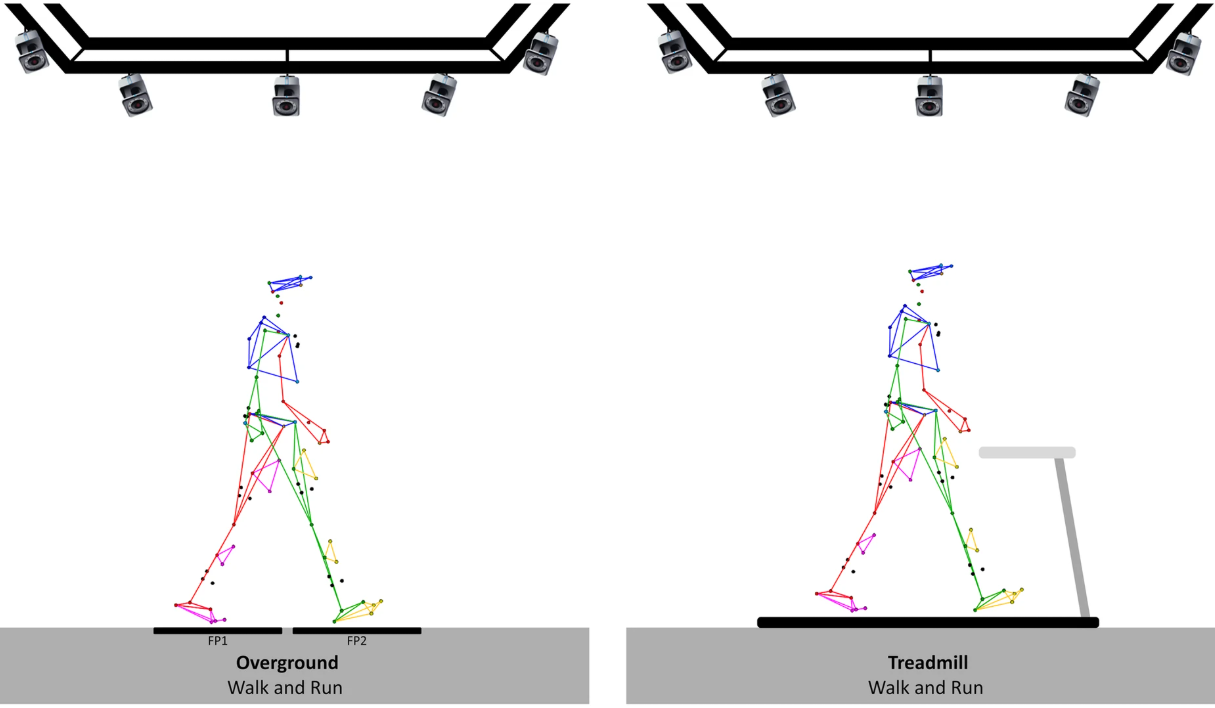
\includegraphics[
		height=0.45\textheight,
		width=0.85\linewidth,
		keepaspectratio
		]{graf/walk_sequence.png}%
	}
\end{frame}



%%%%%%%%%%%%%%%%%%%%%%%%%%%%%%%%%%%%%%%%%%%%%%%%%%%%%%%%%%%%%%%%%%%%%%%%
\begin{frame}[fragile]{Pipeline przetwarzania}
	\begin{itemize}
		\item Wczytanie plików CSV dla uczestników i sesji.
		\item Centrowanie markerów względem miednicy.
		\item Standaryzacja cech.
		\item Podział sygnału na okna czasowe \texttt{window} z krokiem \texttt{step}.
		\item Podział \texttt{train/val/test} typu \texttt{within\_participant}.
	\end{itemize}
\end{frame}


%%%%%%%%%%%%%%%%%%%%%%%%%%%%%%%%%%%%%%%%%%%%%%%%%%%%%%%%%%%%%%%%%%%%%%%%
\begin{frame}[fragile]{Model LSTM i zadania klasyfikacji}
	\begin{itemize}
		\item LSTM modeluje zależności czasowe między kolejnymi klatkami ruchu.
		\item Wejście: tensor \texttt{(window, n\_features)} ze współrzędnymi XYZ markerów.
		\item Wyjście: klasyfikacja przez warstwę softmax.
	\end{itemize}
	
	\vspace{0.5em}
	\textbf{Zadania klasyfikacji:}
	\begin{itemize}
		\item \textbf{\texttt{gait\_type}} -- typ ruchu,
		\item \textbf{\texttt{sex}} -- płeć uczestnika,
		\item \textbf{\texttt{participant\_id}} -- identyfikacja uczestnika.
	\end{itemize}
\end{frame}
	
	
	%%%%%%%%%%%%%%%%%%%%%%%%%%%%%%%%%%%%%%%%%%%%%%%%%%%%%%%%%%%%%%%%%%%%%%%%
	\begin{frame}[fragile]{Siedem konfiguracji modeli (preset \texttt{presentation})}
		\small
		\begin{table}
			\begin{tabular}{lrrlr}
				\toprule
				Nazwa & Okno & Krok & Warstwy LSTM & Dropout \\
				\midrule
				\texttt{win5\_lstm15} & 5 & 5 & 15 & 0.20 \\
				\texttt{win10\_lstm15x15} & 10 & 5 & 15, 15 & 0.20 \\
				\texttt{win20\_lstm15x15x15} & 20 & 10 & 15, 15, 15 & 0.25 \\
				\texttt{win20\_lstm32} & 20 & 10 & 32 & 0.30 \\
				\texttt{win50\_lstm32} & 50 & 25 & 32 & 0.30 \\
				\texttt{win50\_lstm64} & 50 & 25 & 64 & 0.30 \\
				\texttt{win100\_lstm64x32\_dense32} & 100 & 50 & 64, 32 (+Dense 32) & 0.30 \\
				\bottomrule
			\end{tabular}
		\end{table}
		
		\vspace{0.5em}
		\begin{block}{Skala eksperymentu}
			7 konfiguracji $\times$ 3 zadania = \textbf{21 wytrenowanych modeli}, optymalizator Adam (lr = 0{,}001)
		\end{block}
	\end{frame}
	
	
	%%%%%%%%%%%%%%%%%%%%%%%%%%%%%%%%%%%%%%%%%%%%%%%%%%%%%%%%%%%%%%%%%%%%%%%%
	\begin{frame}[fragile]{Kod -- skrypt treningowy}
		\textbf{\texttt{scripts/train\_lstm\_experiments.py}}
		
		\begin{itemize}
			\item Dla każdej konfiguracji i każdego zadania:
			\begin{itemize}
				\item wczytuje dane, buduje okna i podział train/val/test,
				\item budowa modelu: stacked LSTM + (opcjonalnie Dense) + warstwa wyjściowa softmax,
				\item trening z \texttt{EarlyStopping} / checkpointami -- zapis \texttt{best\_model.keras} (wg \texttt{val\_loss}) i \texttt{last\_model.keras},
				\item ewaluacja na poziomie \textbf{okna} oraz \textbf{całego nagrania} (agregacja predykcji okien przez modę).
			\end{itemize}
			\item Wyniki zapisywane do \texttt{models/lstm\_experiments/<run>/}:\\
			\texttt{history.csv}, \texttt{metrics.json}, \texttt{*\_predictions.csv}, \texttt{*\_confusion\_matrix.csv/.png}.
		\end{itemize}
	\end{frame}
	
	
	%%%%%%%%%%%%%%%%%%%%%%%%%%%%%%%%%%%%%%%%%%%%%%%%%%%%%%%%%%%%%%%%%%%%%%%%
	\begin{frame}[fragile]{Metryki ewaluacji}
		\begin{itemize}
			\item \textbf{Poziom okna} -- predykcja dla pojedynczego okna czasowego.
			\item \textbf{Poziom nagrania} -- agregacja predykcji okien danego pliku przez \textbf{modę} -> jedna finalna decyzja na nagranie.
			\item Metryki: \texttt{accuracy}, \texttt{precision}, \texttt{recall}, \texttt{F1-macro}, macierz pomyłek.
			\item \texttt{F1-macro} jako główna metryka rankingowa -- odporna na nierównowagę klas (istotne zwłaszcza dla \texttt{participant\_id}).
		\end{itemize}
		
		\begin{block}{Schemat agregacji okno -> nagranie}
			każde nagranie dzielone jest na okna -> model klasyfikuje każde okno -> wynik nagrania = klasa najczęściej przewidywana wśród jego okien
		\end{block}
	\end{frame}
	
		%%%%%%%%%%%%%%%%%%%%%%%%%%%%%%%%%%%%%%%%%%%%%%%%%%%%%%%%%%%%%%%%%%%%%%%%
	\begin{frame}[fragile]{Wyniki -- typ chodu}
		\begin{itemize}
			\item Najtrudniejsze zadanie i jedyne z realną rywalizacją modeli.
			\item Poziom nagrania: trzy konfiguracje remisują w okolicy 83--84\%:
			\begin{itemize}
				\item \texttt{win20\_lstm32} -- \textbf{84,0\%} (najlepszy),
				\item \texttt{win10\_lstm15x15} -- 83,7\%,
				\item \texttt{win50\_lstm64} -- 83,2\%.
			\end{itemize}
			\item Poziom okna: zdecydowanie wygrywa \texttt{win50\_lstm64} -- 76,3\%.
			\item Wybór modelu zależy od jednostki decyzji: całe nagranie -> \texttt{win20\_lstm32}; pojedyncze okno (np. real-time) -> \texttt{win50\_lstm64}.
		\end{itemize}
	\end{frame}
	
		%%%%%%%%%%%%%%%%%%%%%%%%%%%%%%%%%%%%%%%%%%%%%%%%%%%%%%%%%%%%%%%%%%%%%%%%
	\begin{frame}[fragile]{Wyniki -- typ chodu (porównanie modeli)}
		\centering
		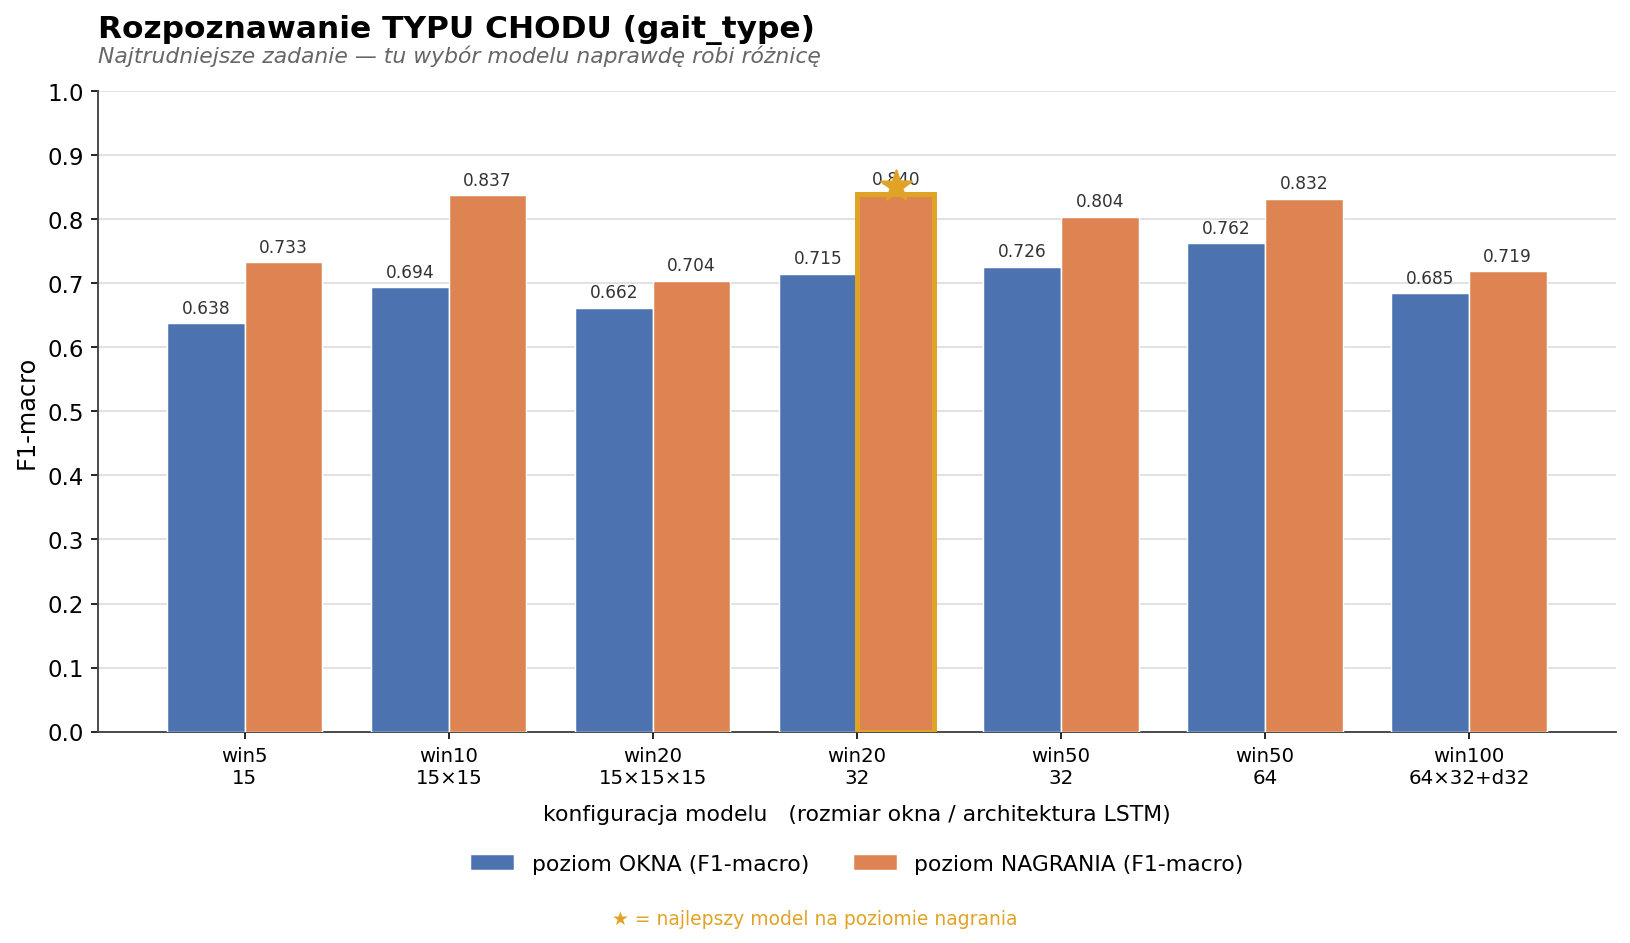
\includegraphics[height=0.95\textheight, keepaspectratio]{graf/model_comparison_f1gait.png}
	\end{frame}
	
	%%%%%%%%%%%%%%%%%%%%%%%%%%%%%%%%%%%%%%%%%%%%%%%%%%%%%%%%%%%%%%%%%%%%%%%%
	\begin{frame}[fragile]{Wyniki -- typ chodu (macierz pomyłek)}	
		\centering
		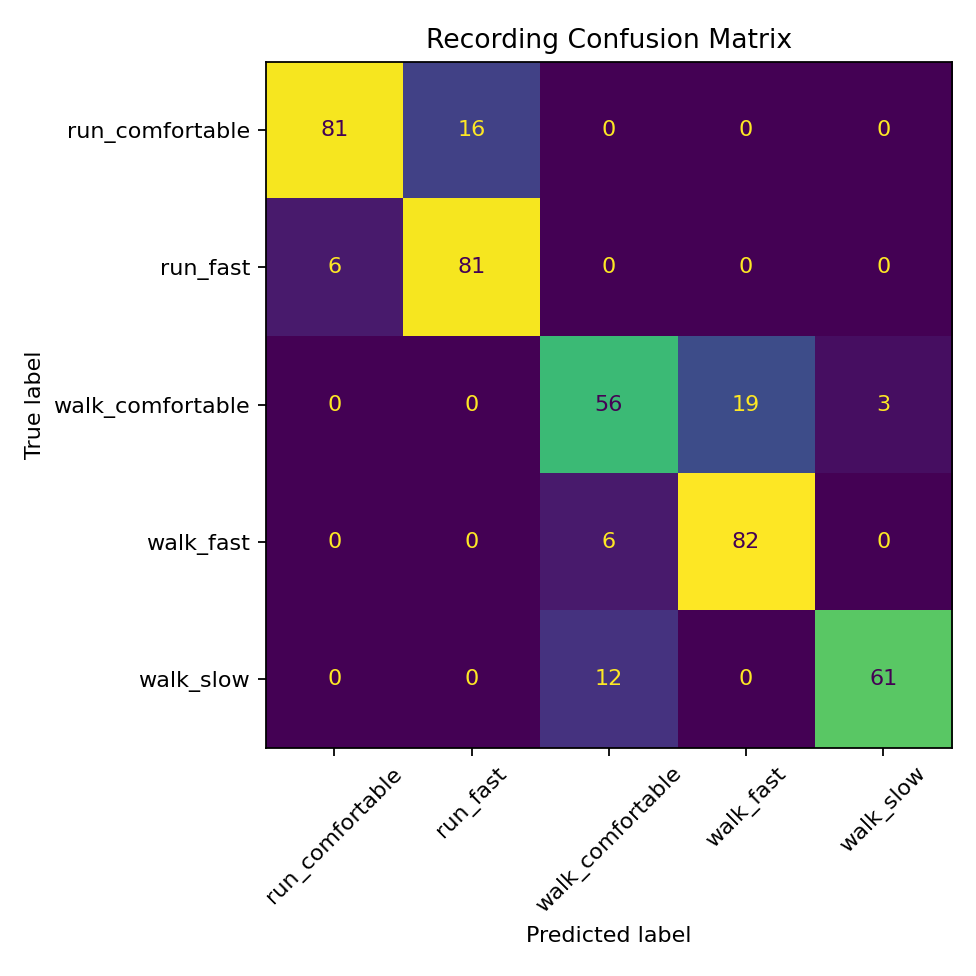
\includegraphics[width=0.55\textwidth]{graf/gait_type_confusion_matrix.png}
		
	\end{frame}
	
	%%%%%%%%%%%%%%%%%%%%%%%%%%%%%%%%%%%%%%%%%%%%%%%%%%%%%%%%%%%%%%%%%%%%%%%%
	\begin{frame}[fragile]{Wyniki -- rozpoznawanie płci}
		\begin{itemize}
			\item Wszystkie 7 konfiguracji, łącznie z najmniejszą (\texttt{win5\_lstm15}), osiągają \textbf{accuracy / F1-macro $\approx$ 100\%}.
			\item Zarówno na poziomie okna, jak i całego nagrania.
			\item Różnice anatomiczne między płciami są na tyle wyraźne, że nawet bardzo prosty model je wychwytuje.
		\end{itemize}
	\end{frame}
	
		
	%%%%%%%%%%%%%%%%%%%%%%%%%%%%%%%%%%%%%%%%%%%%%%%%%%%%%%%%%%%%%%%%%%%%%%%%
	\begin{frame}[fragile]{Wyniki -- rozpoznawanie płci (porównanie modeli)}
		\centering
		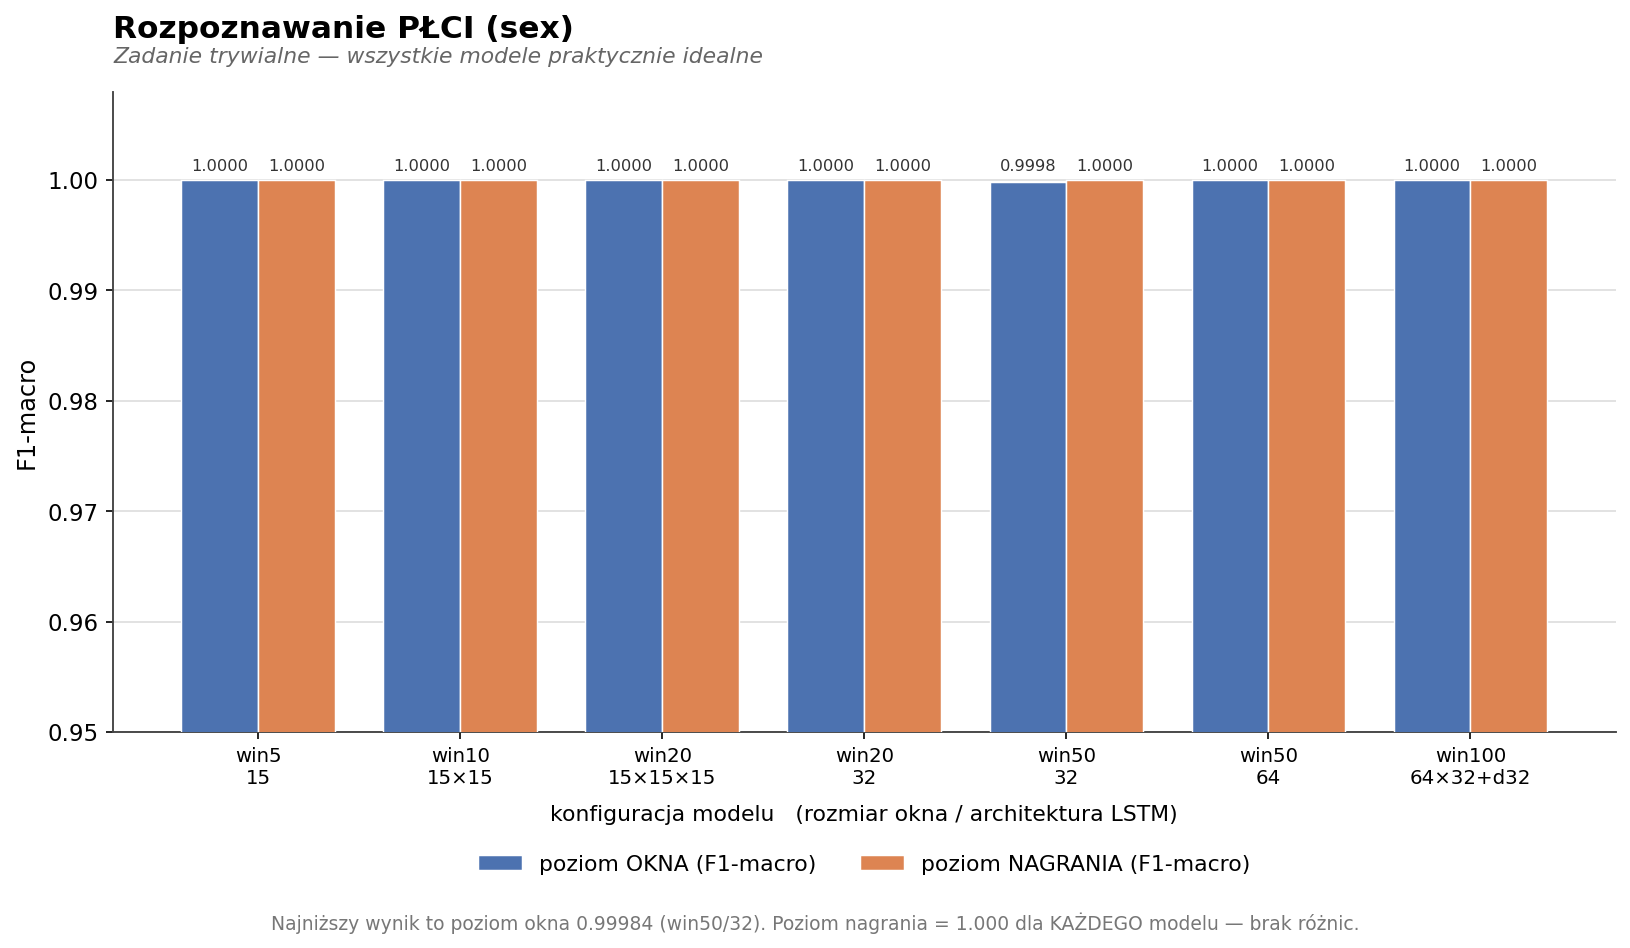
\includegraphics[height=0.95\textheight, keepaspectratio]{graf/model_comparison_f1sex.png}
	\end{frame}
	
	
	
		%%%%%%%%%%%%%%%%%%%%%%%%%%%%%%%%%%%%%%%%%%%%%%%%%%%%%%%%%%%%%%%%%%%%%%%%
	\begin{frame}[fragile]{Wyniki -- rozpoznawanie płci (macierz pomyłek)}
		\centering
		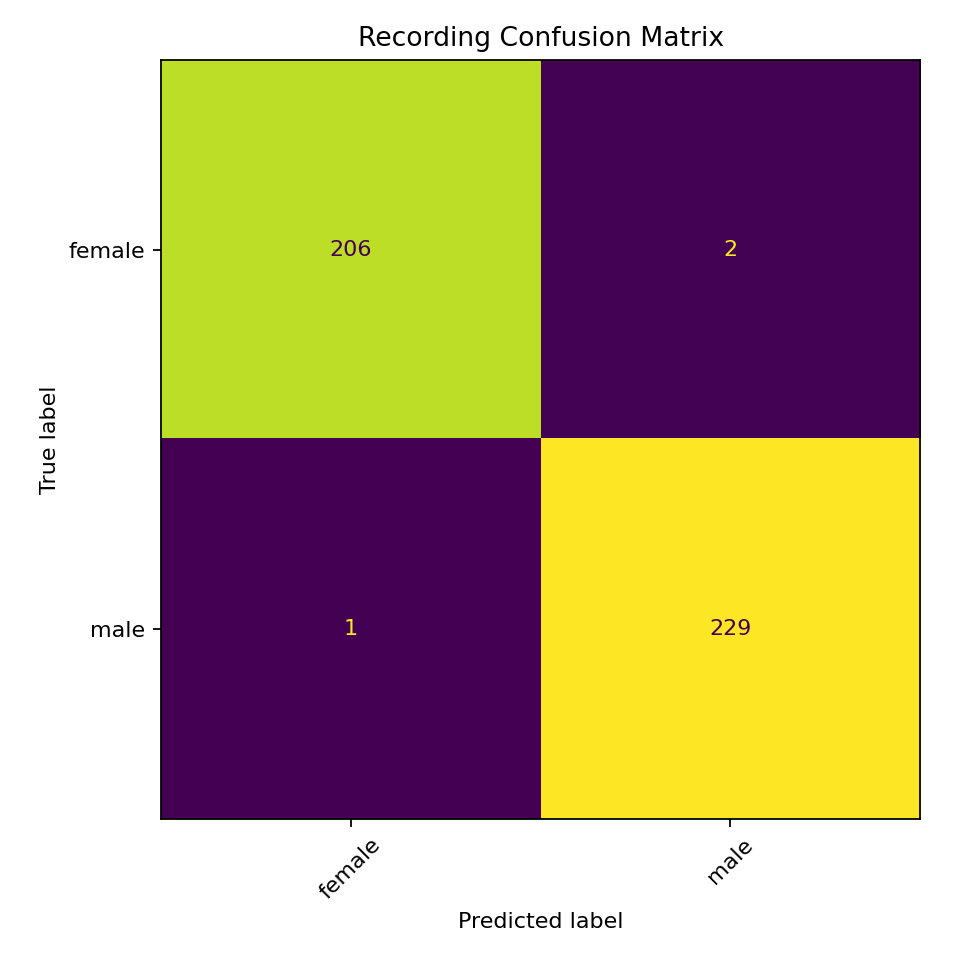
\includegraphics[width=0.55\textwidth]{graf/sex_confusion_matrix.png}
		
	\end{frame}
	

	
	%%%%%%%%%%%%%%%%%%%%%%%%%%%%%%%%%%%%%%%%%%%%%%%%%%%%%%%%%%%%%%%%%%%%%%%%
	\begin{frame}[fragile]{Wyniki -- identyfikacja uczestnika}
		\begin{itemize}
			\item Obraz \textbf{dwubiegunowy}: część konfiguracji prawie idealna, część ,,zapada się''.
			\item \texttt{win10\_lstm15x15} i \texttt{win50\_lstm64}: \textbf{100\% accuracy / F1} na poziomie nagrania.
			\item Słabsze modele (\texttt{win5\_lstm15}, \texttt{win20\_lstm32}, \texttt{win50\_lstm32}): spadek do $\sim$75\% na nagraniu.
			\item Ciekawy efekt: dla słabych modeli wynik na poziomie \textbf{okna bywa wyższy} niż na poziomie nagrania (\texttt{win50\_lstm32}: 84{,}4\% okno vs 75{,}6\% nagranie) -- błędy nie są losowe, całe nagrania trafiają do złej klasy.
		\end{itemize}
	\end{frame}
	
		%%%%%%%%%%%%%%%%%%%%%%%%%%%%%%%%%%%%%%%%%%%%%%%%%%%%%%%%%%%%%%%%%%%%%%%%
	\begin{frame}[fragile]{Wyniki -- identyfikacja uczestnika (porównanie modeli)}
		\centering
		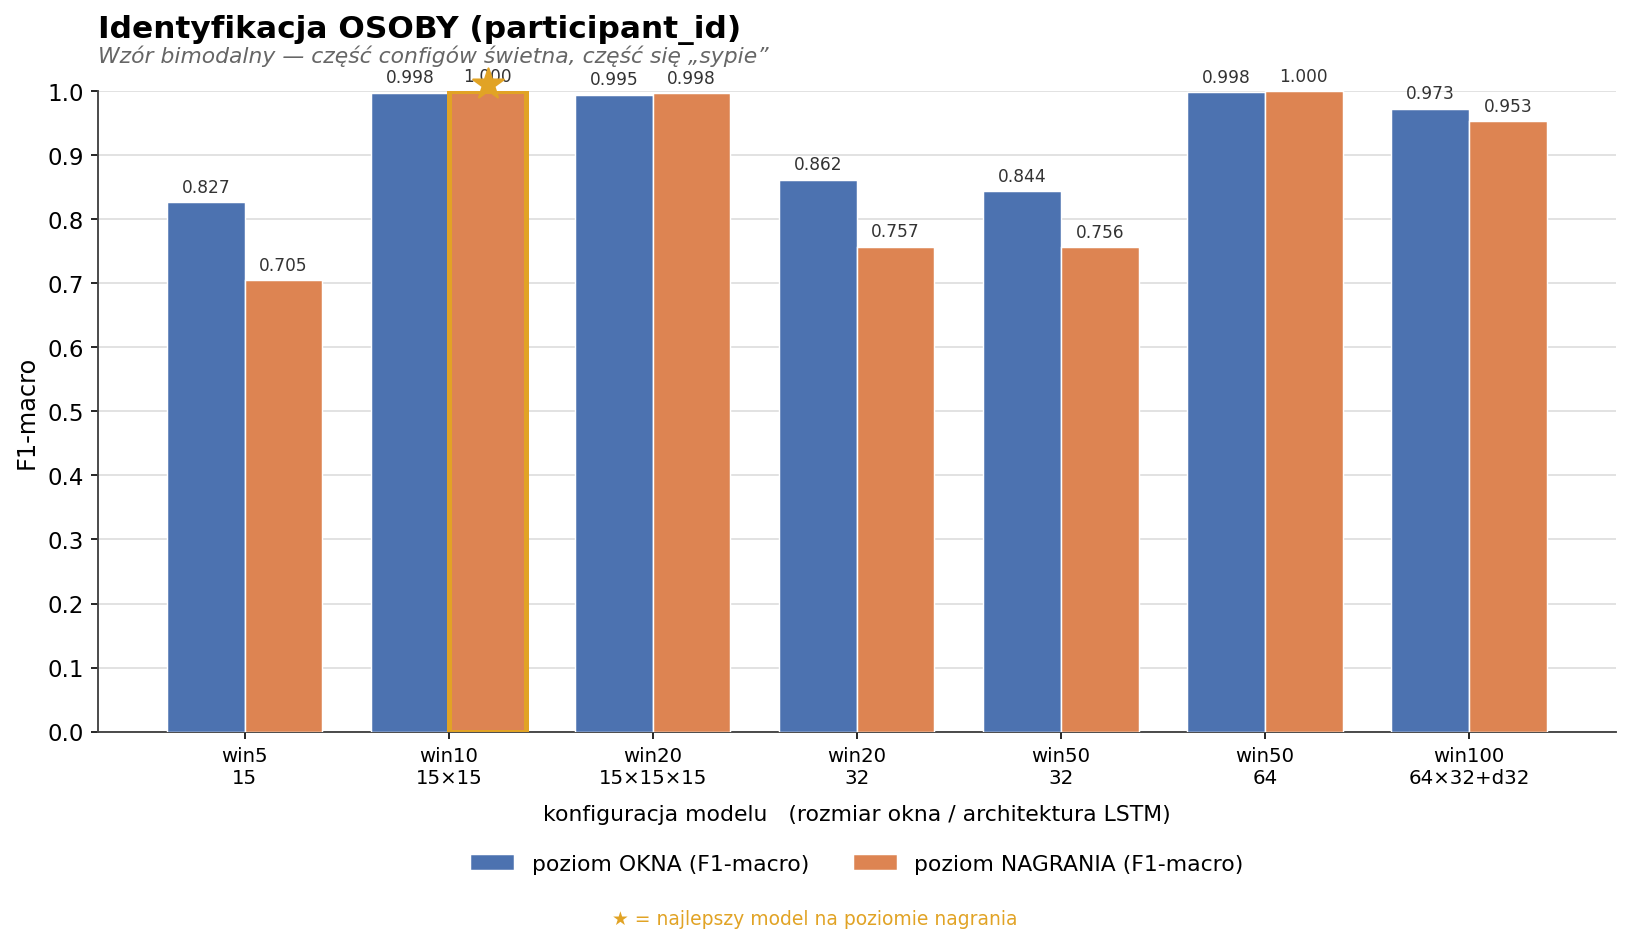
\includegraphics[height=0.95\textheight, keepaspectratio]{graf/model_comparison_f1id.png}
	\end{frame}
	
	
	%%%%%%%%%%%%%%%%%%%%%%%%%%%%%%%%%%%%%%%%%%%%%%%%%%%%%%%%%%%%%%%%%%%%%%%%
	\begin{frame}[fragile]{Wyniki -- identyfikacja uczestnika (macierz pomyłek)}

		\centering
		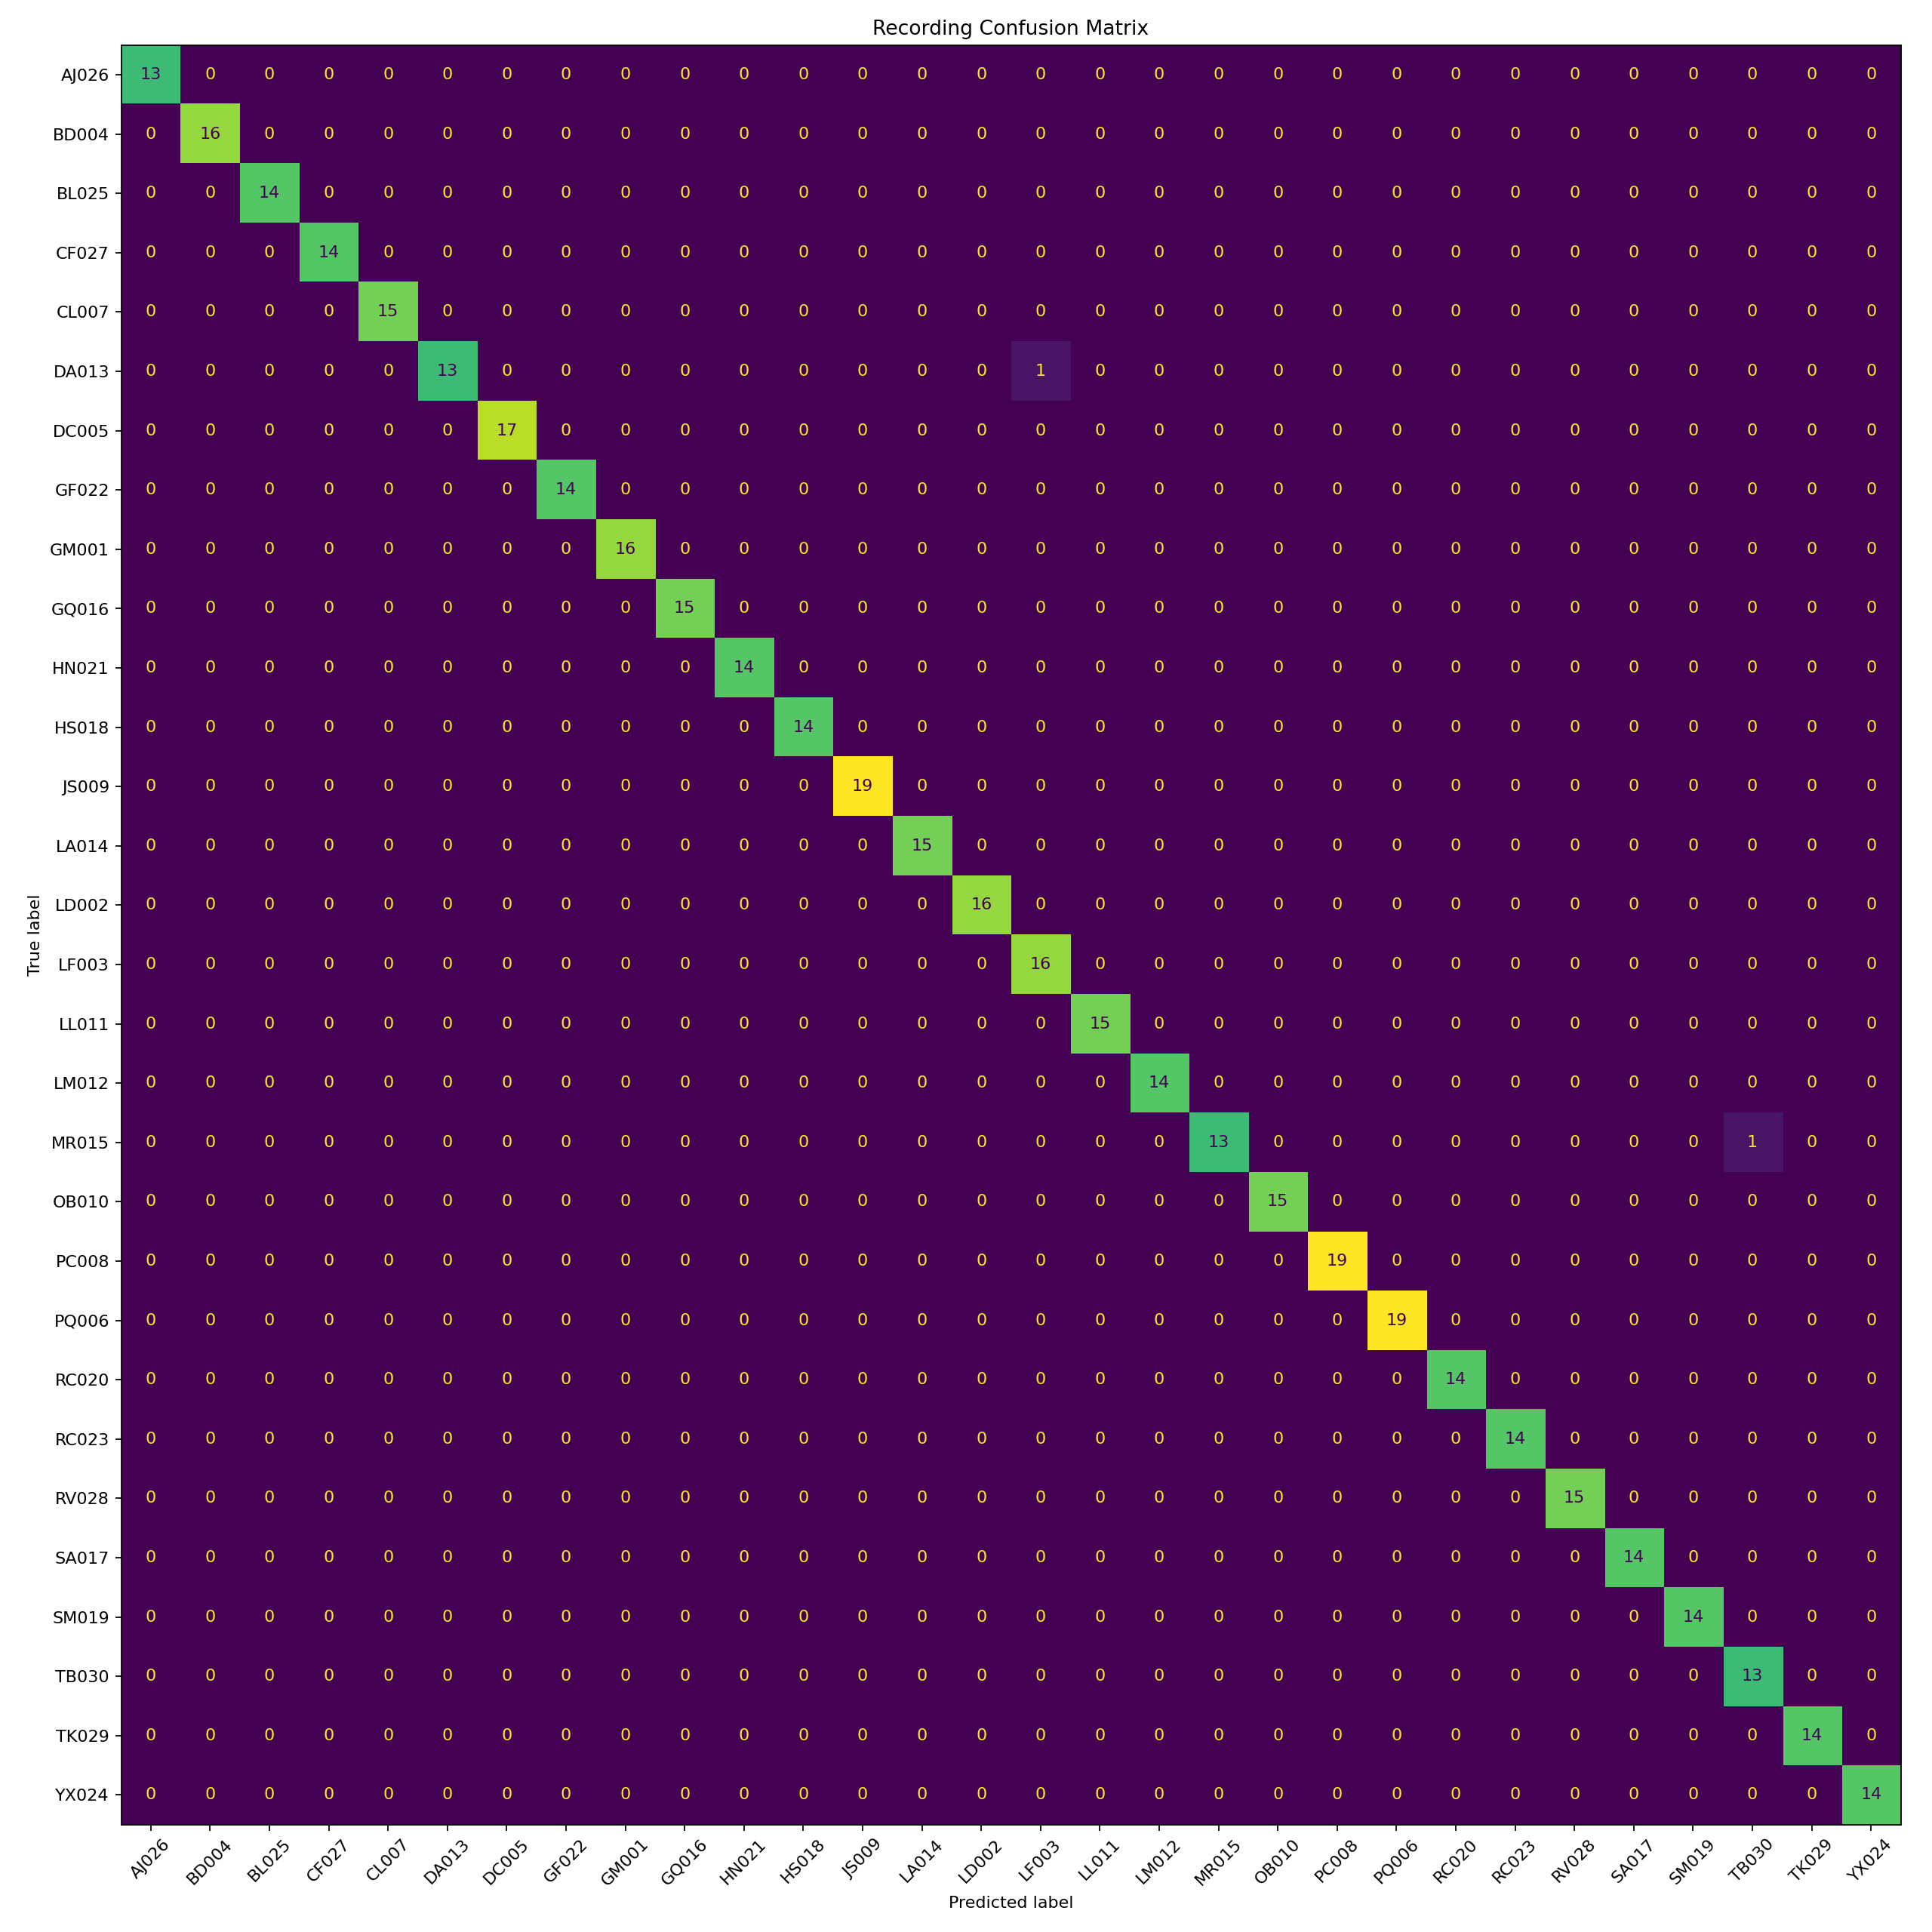
\includegraphics[width=0.55\textwidth]{graf/participant_id_confusion_matrix.png}

	\end{frame}
	


	
	%%%%%%%%%%%%%%%%%%%%%%%%%%%%%%%%%%%%%%%%%%%%%%%%%%%%%%%%%%%%%%%%%%%%%%%%
	\begin{frame}[fragile]{Podsumowanie wyników}
		\small
		\begin{table} 
			\centering \scriptsize 
			\begin{tabular}
				{@{}lccc@{}} \toprule Zadanie & Okno & Nagranie & F1 \\ 
				\midrule Chód & w50-L64: 76,3\% & w20-L32: 84,0\% & $\sim$0,84 \\ 
				Płeć & $\sim$100\% & 100\% & 1,00 \\ ID & w50-L64: 99,8\% & w10-L15x2 / w50-L64: 100\% & 1,00 \\ 
				\bottomrule 
			\end{tabular} 
		\end{table}
		
		\vspace{0.8em}
		\begin{block}{Wniosek praktyczny}
			\texttt{win50\_lstm64} jest najbezpieczniejszym wyborem ,,uniwersalnym'' -- wygrywa lub remisuje na poziomie okna we wszystkich trzech zadaniach.
		\end{block}
	\end{frame}
	
	
	%%%%%%%%%%%%%%%%%%%%%%%%%%%%%%%%%%%%%%%%%%%%%%%%%%%%%%%%%%%%%%%%%%%%%%%%
	\begin{frame}[fragile]{Hipoteza: overfitting dla \texttt{sex} i \texttt{participant\_id}}
		\begin{itemize}
			\item Oczekiwania (z literatury / planu projektu): typ chodu $>$95\%, płeć 80--90\%, identyfikacja uczestnika 70--85\%.
			\item Rzeczywiste wyniki: typ chodu $\sim$87\% accuracy (84\% F1), płeć i ID uczestnika -- \textbf{100\%}.
			\item Tak wysoki wynik dla zadań ,,trudniejszych z definicji'' jest podejrzany i może sugerować overfitting
			\item Możliwe przyczyny:
			\begin{itemize}
				\item podział \texttt{within\_participant} -- okna z tego samego nagrania (bardzo podobne) trafiają zarówno do train, jak i do test,
				\item sieć może uczyć się ,,sygnatury'' konkretnego nagrania/uczestnika (np. wzrost, proporcje ciała widoczne w pozycjach markerów) zamiast uogólnionego wzorca,
			\end{itemize}
		\end{itemize}
	\end{frame}
	
	
	%%%%%%%%%%%%%%%%%%%%%%%%%%%%%%%%%%%%%%%%%%%%%%%%%%%%%%%%%%%%%%%%%%%%%%%%
	\begin{frame}[fragile]{Wnioski z projektu}
		\begin{itemize}
			\item Sieci LSTM dobrze radzą sobie z klasyfikacją danych mocap na podstawie okien czasowych współrzędnych markerów.
			\item Agregacja okno -> nagranie zwykle poprawia wynik, ale nie zawsze -- przy słabych modelach może go pogorszyć.
			\item Wynik silnie zależy od zadania: typ chodu jest istotnie trudniejszy niż płeć czy identyfikacja uczestnika.
			\item Najlepszy ,,uniwersalny'' model w naszych eksperymentach: \texttt{win50\_lstm64}.
			\item 100\% trafności dla płci i ID uczestnika wymaga dalszej weryfikacji (np. podział \texttt{participant\_holdout}, walidacja na zupełnie nowych uczestnikach).
		\end{itemize}
	\end{frame}
	
	
	%%%%%%%%%%%%%%%%%%%%%%%%%%%%%%%%%%%%%%%%%%%%%%%%%%%%%%%%%%%%%%%%%%%%%%%%
	\begin{frame}[fragile]{Literatura i~źródła}
		\textbf{Artykuł referencyjny:}
		\begin{itemize}
			\item da Silva, R., Ondřej, J., Smolic, A.\\
			\emph{Using LSTM for Automatic Classification of Human Motion Capture Data}.\\
			VISIGRAPP 2019, s.~236--243.\\
			DOI: \texttt{10.5220/0007349902360243}
		\end{itemize}
		
		\vspace{0.8em}
		\textbf{Zbiór danych:}
		\begin{itemize}
			\item Riglet, L. i~in.\\
			\emph{3D motion analysis dataset of healthy young adult volunteers walking and running on overground and treadmill}.\\
			Scientific Data 11, 556 (2024).\\
			\url{https://www.nature.com/articles/s41597-024-03420-y}
		\end{itemize}
	\end{frame}
	
\end{document}